\newpage
\section{Launch Phase}
\subsection{General Analysis}
	\subsubsection{Requirements	 Analysis}
		Put in description of the requirements... \textbf{JESUS}
		\begin{itemize}
			\item Functional Requirements ("system shall do 'requirement' ")
			\item Non-functional Requirements ("system shall be 'requirement' ")
			\item Behavioural Requirements ("how the system shall react")
			\item Performance Requirements ("how well does it have to be done")
		\end{itemize}
		\begin{figure}[h!]		%Remember to put the h!, to not fuck the sections.
			\begin{centering}
				 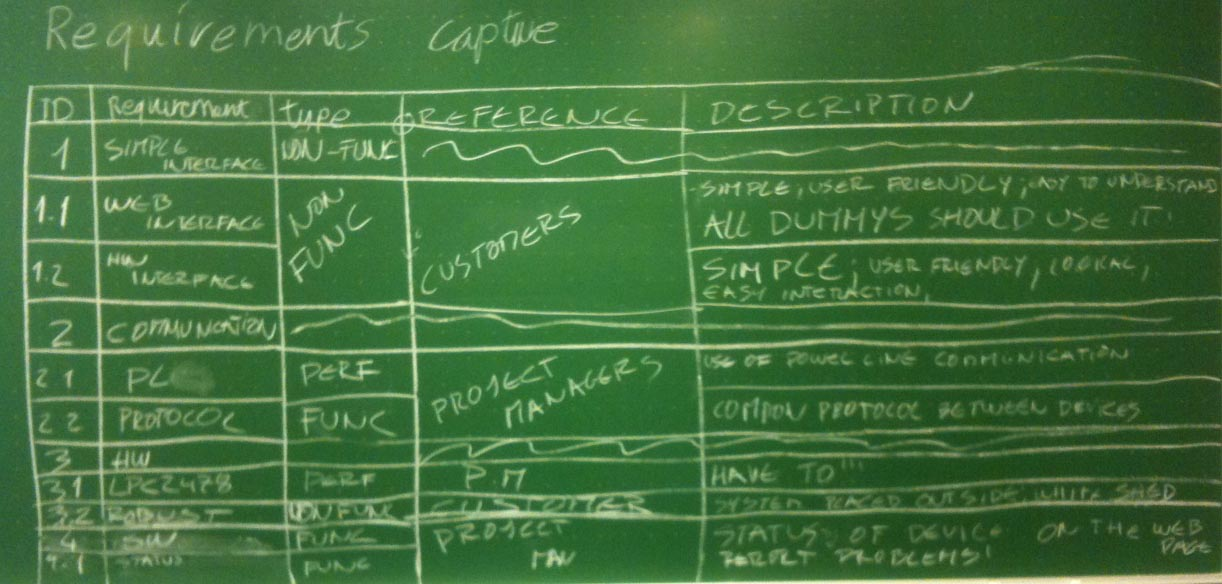
\includegraphics[width=1.0\textwidth]{images/requirement_capture.JPG}
		 		\caption{Design}
			 \end{centering}
		\end{figure}
	\subsubsection{Problem Domain Analysis}
			\paragraph{Block Diagram:}
				\textbf{Candidates in the system}
				\\\textbf{Consumers:} Units that consumes power (e.g. light, washing machine, electric car)
				\\\textbf{Producers:} Modules that delivers energy to the hub (e.g. Wind-turbine, photovoltaic-cells)
				\\\textbf{Storage:} Modules that both consumes when the system over produces and "produces" (gives energy to the consumers) when needed. 
				\\\textbf{Temperature:} Unit that measures the outdoor temperature. If the temperature is too high or low it might damage the hardware.
				\\\textbf{Humidity:} Unit that measures the humidity where the system is places. If the humidity is too high.
				\newline
			\paragraph{Block Diagram:}
				\textbf{Event in the system}
				\\\textbf{TemperatureBelowLimit}
				\\\textbf{TemperatureAboveLimit}
				\\\textbf{HumidityAboveLimit}
				\\\textbf{EnergyAboveLimit}
				\\\textbf{EnergyBelowLimit}
				\\\textbf{InitModule}
				\\\textbf{StartModule}
				\\\textbf{StopModule}
				\\\textbf{StandbyModule}
				\\
				\begin{table}[h!]
					\begin{tabular}{| r | c | c | c | c | c |}
					\hline
					~ & Consumers & Producers & Storage & Temp & Humidity \\ \hline
					TempBellowLimit & ~ & ~ & ~ & X & ~ \\ \hline
					TempAboveLimit & ~ & ~ & ~ & X & ~ \\ \hline
					HumidityAboveLimit & ~ & ~ & ~ & ~ & X \\ \hline
					InitModule & X & X & X & ~ & ~ \\ \hline
					StartModule & X & X & X & ~ & ~ \\ \hline
					StopModule & X & X & X & ~ & ~ \\ \hline
					StandbyModule & ~ & X & X & ~ & ~ \\ \hline
					EnergyAboveLimit & ~ & X & ~ & ~ & ~ \\ \hline
					EnergyBelowLimit & ~ & X & ~ & ~ & ~ \\
					\hline
					\end{tabular}
				\end{table}
				\\ Text about all different states in the system.  \textbf{DENNES}
				\\\textbf{Table with all the above candidates and event combined:}
				\newline
			\paragraph{State Machine Diagrams}
			 \textbf{DENNES}
	\subsubsection{Usage Domain Analysis}
		\begin{itemize}
			\item Use Cases - Put in diagrams of user + system (modules)
		\end{itemize}
	\subsubsection{Interface Analysis}
			Put in the comic book story!  \textbf{JESUS}
		\begin{itemize}
			\item User Interface Descriptions
				
			\item System Interface Descriptions
		\end{itemize}
	\subsubsection{Function Analysis}
	 \textbf{THIS}
		\begin{itemize}
			\item Recognise the direction of the device ( input, output, both ).
			\item Start / Stop slave devices from web interface or physical module ( Control over the connected modules ).
			\item Routes energy from the input to output ports.
			\item Control power status of slave modules.
			\item Log device data ( uptime of the port and power amount since connected ).
			\item More to add here...
		\end{itemize}
	\subsubsection{System Dynamics}
			Put in example from eudp: %eudp.dk/index.php/Sequence_Diagrams
			 \textbf{JESUS / DENNES}
		\begin{itemize}
			\item Communication Diagram
			\item Sequence Diagram
		\end{itemize}
	\subsubsection{General Analysis Specification}
		 \textbf{THIS}
\subsection{General Architecture Design}
	\subsubsection{Design Criteria}
		Write in what parts should be used (mostly off the shelf things).  \textbf{THIS}
	\subsubsection{Subsystem Design}
		\begin{itemize}
			\item Subsystem Architecture Diagram
			\item Detailed Block Diagrams
		\end{itemize}
	\subsubsection{Architecture Dynamics}
		Hubs communication with submodules
		\begin{itemize}
			\item Sequence Diagrams
		\end{itemize}
	\subsubsection{Architectural Specification and Constraints}
\subsection{Technical Platform}
	A lot of technical stuffs. 
	\subsubsection{Hardware Specifications}
	\subsubsection{Software Specifications}